\documentclass[11pt,a4paper]{article}
\usepackage[utf8]{inputenc}
\usepackage[margin=1in]{geometry}
\usepackage{amsmath}
\usepackage{hyperref}
\usepackage{listings}
\usepackage{xcolor}
\usepackage{tikz}
\usetikzlibrary{shapes,arrows,positioning,decorations.pathreplacing}

\title{Zed's Smart Edit Architecture: A Unified Approach to AI-Powered Code Editing}
\author{Research Paper}
\date{\today}

\begin{document}

\maketitle

\section{Introduction}

Smart edit refers to the ability of a code editor to automatically apply changes to files when a user requests modifications through a language model interface. Unlike traditional code completion, smart edit allows users to describe desired changes in natural language, and the system intelligently determines which code to modify and safely applies edits, often across multiple files.

This paper examines how Zed, a modern code editor, implements smart edit functionality through its Agent Panel chat interface. We focus specifically on how the system handles three distinct scenarios: online language models, offline models with tool calling capabilities, and offline models without tool calling support.

\section{Unified Smart Edit Pipeline}

Zed's smart edit system is built around a unified architecture that handles all three model types through a single pipeline. The core components are:

\begin{itemize}
    \item \textbf{Agent Panel}: The chat interface where users interact with language models
    \item \textbf{EditFileTool}: A tool that validates paths, opens buffers, and manages the editing process
    \item \textbf{EditAgent}: The component that renders prompts, parses model responses, and applies edits
    \item \textbf{Edit Parser}: Handles parsing of structured edit formats (XML tags or diff-fenced blocks)
    \item \textbf{Streaming Fuzzy Matcher}: Matches edit instructions against actual file content
\end{itemize}

The pipeline works as follows: when a user requests a change in the Agent Panel, the model (if tool-capable) calls the \texttt{edit\_file} tool. This tool validates the file path, opens the buffer, and delegates to EditAgent. EditAgent renders a prompt template specific to the model's preferred format, sends it to the model, and streams the response back. The response is parsed into structured edits, matched against the buffer using fuzzy matching, and applied incrementally while showing a diff UI to the user.

\begin{figure}[htbp]
\centering
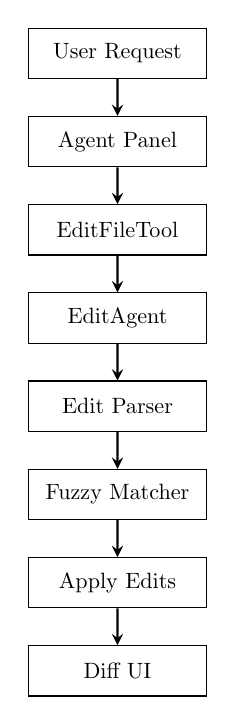
\begin{tikzpicture}[
    node distance=1.4cm,
    box/.style={rectangle, draw, text width=2.6cm, text centered, minimum height=0.8cm},
    arrow/.style={->, >=stealth, thick},
    scale=0.8,
    transform shape
]
    \node[box] (user) {User Request};
    \node[box, below of=user] (panel) {Agent Panel};
    \node[box, below of=panel] (tool) {EditFileTool};
    \node[box, below of=tool] (agent) {EditAgent};
    \node[box, below of=agent] (parser) {Edit Parser};
    \node[box, below of=parser] (matcher) {Fuzzy Matcher};
    \node[box, below of=matcher] (apply) {Apply Edits};
    \node[box, below of=apply] (diff) {Diff UI};

    \draw[arrow] (user) -- (panel);
    \draw[arrow] (panel) -- (tool);
    \draw[arrow] (tool) -- (agent);
    \draw[arrow] (agent) -- (parser);
    \draw[arrow] (parser) -- (matcher);
    \draw[arrow] (matcher) -- (apply);
    \draw[arrow] (apply) -- (diff);
\end{tikzpicture}
\caption{Unified Smart Edit Pipeline Architecture}
\label{fig:pipeline}
\end{figure}

\section{Online Language Models}

Online models include hosted providers such as OpenAI, Anthropic, Google AI, and GitHub Copilot. These models run in the cloud and are accessed via HTTPS with API keys.

\subsection{How It Works}

When using an online model with tool calling support, the flow is straightforward:

\begin{enumerate}
    \item User types a request in the Agent Panel (e.g., "Add error handling to the login function")
    \item The model receives the conversation context, including available tools
    \item The model calls the \texttt{edit\_file} tool with a path and description
    \item EditFileTool validates the path, opens the buffer, and creates a diff view
    \item EditAgent renders a prompt template (XML tags for most models, diff-fenced for Gemini)
    \item The model streams back structured edits in the chosen format
    \item The parser extracts \texttt{<old\_text>} and \texttt{<new\_text>} pairs (or diff markers)
    \item The fuzzy matcher locates the old text in the buffer
    \item Edits are applied incrementally and shown in a diff drawer
    \item User reviews and accepts or rejects changes
\end{enumerate}

The key advantage of online models is their high quality and full tool-use support. Models like Claude and GPT-4 can reason about multi-file changes, search the codebase, and apply complex edits. However, this comes with latency and cost, and data leaves the local machine.

\begin{figure}[htbp]
\centering
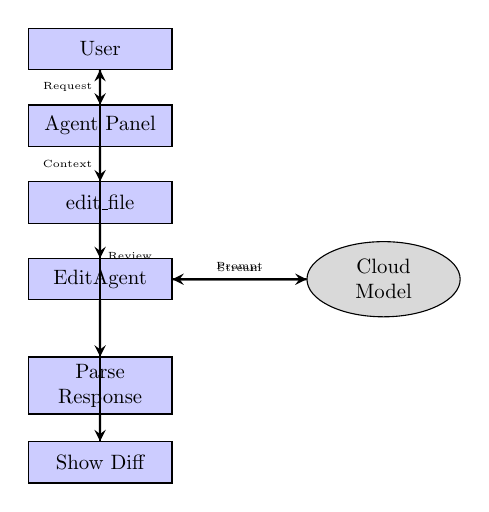
\begin{tikzpicture}[
    node distance=1.3cm,
    box/.style={rectangle, draw, text width=2.2cm, text centered, minimum height=0.7cm, fill=blue!20},
    cloud/.style={ellipse, draw, text width=1.6cm, text centered, minimum height=0.8cm, fill=gray!30},
    arrow/.style={->, >=stealth, thick},
    scale=0.75,
    transform shape
]
    \node[box] (user) {User};
    \node[box, below of=user] (panel) {Agent Panel};
    \node[box, below of=panel] (tool) {edit\_file};
    \node[box, below of=tool] (agent) {EditAgent};
    \node[cloud, right of=agent, xshift=3.5cm] (model) {Cloud Model};
    \node[box, below of=agent, yshift=-0.5cm] (parse) {Parse Response};
    \node[box, below of=parse] (diff) {Show Diff};

    \draw[arrow] (user) -- node[left, font=\tiny] {Request} (panel);
    \draw[arrow] (panel) -- node[left, font=\tiny] {Context} (tool);
    \draw[arrow] (tool) -- (agent);
    \draw[arrow] (agent) -- node[above, font=\tiny] {Prompt} (model);
    \draw[arrow] (model) -- node[above, font=\tiny] {Stream} (agent);
    \draw[arrow] (agent) -- (parse);
    \draw[arrow] (parse) -- (diff);
    \draw[arrow] (diff) -- node[right, font=\tiny] {Review} (user);
\end{tikzpicture}
\caption{Online Model Flow with Tool Calling}
\label{fig:online}
\end{figure}

\subsection{Provider Abstraction}

Zed uses a provider abstraction layer that allows the Agent Panel to swap models mid-conversation, inspect tool calls, and display token usage without vendor-specific code. This means the same smart edit flow works whether using OpenAI, Anthropic, or any other supported provider.

\section{Offline Models With Tool Calls}

Offline models with tool calling support include self-hosted solutions like Ollama, LM Studio, or custom gateways that expose OpenAI-compatible APIs. These models run entirely on the user's machine or local network.

\subsection{Architecture}

The architecture for offline tool-capable models is nearly identical to online models. The main difference is that the model endpoint is local (e.g., \texttt{http://localhost:11434} for Ollama). Zed doesn't distinguish between local and remote endpoints at the protocol level.

\subsection{Implementation Details}

When a local model advertises \texttt{supports\_tools: true}, Zed attaches tool schemas to requests. The model can then call tools like \texttt{read\_file}, \texttt{list\_directory}, and \texttt{edit\_file} just like online models. The EditAgent uses the same prompt templates and parsing logic.

A key implementation detail is how Zed handles tool choice. When a model reports \texttt{supports\_tool\_choice(LanguageModelToolChoice::None)}, Zed attaches tool definitions but forces the initial call to be a normal response. This allows caching and safety checks to work even if the gateway throttles full tool streaming.

\subsection{Advantages}

Offline models with tool calls provide the best of both worlds: full autonomy (the model can read files, search, and edit) while keeping all data and computation local. This is ideal for privacy-sensitive environments or when working with proprietary codebases.

\begin{figure}[htbp]
\centering
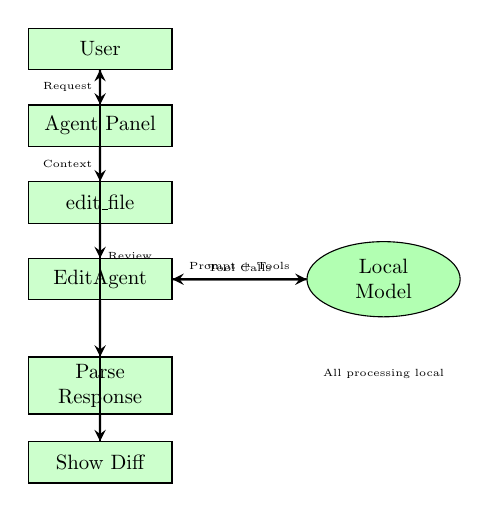
\begin{tikzpicture}[
    node distance=1.3cm,
    box/.style={rectangle, draw, text width=2.2cm, text centered, minimum height=0.7cm, fill=green!20},
    local/.style={ellipse, draw, text width=1.6cm, text centered, minimum height=0.8cm, fill=green!30},
    arrow/.style={->, >=stealth, thick},
    scale=0.75,
    transform shape
]
    \node[box] (user) {User};
    \node[box, below of=user] (panel) {Agent Panel};
    \node[box, below of=panel] (tool) {edit\_file};
    \node[box, below of=tool] (agent) {EditAgent};
    \node[local, right of=agent, xshift=3.5cm] (model) {Local Model};
    \node[box, below of=agent, yshift=-0.5cm] (parse) {Parse Response};
    \node[box, below of=parse] (diff) {Show Diff};

    \draw[arrow] (user) -- node[left, font=\tiny] {Request} (panel);
    \draw[arrow] (panel) -- node[left, font=\tiny] {Context} (tool);
    \draw[arrow] (tool) -- (agent);
    \draw[arrow] (agent) -- node[above, font=\tiny] {Prompt + Tools} (model);
    \draw[arrow] (model) -- node[above, font=\tiny] {Tool Calls} (agent);
    \draw[arrow] (agent) -- (parse);
    \draw[arrow] (parse) -- (diff);
    \draw[arrow] (diff) -- node[right, font=\tiny] {Review} (user);
    
    \node[below of=model, yshift=-0.3cm, text width=2.2cm, text centered, font=\tiny] {All processing local};
\end{tikzpicture}
\caption{Offline Model Flow with Tool Calling}
\label{fig:offline-tools}
\end{figure}

\section{Offline Models Without Tool Calls}

Some local models, particularly smaller ones (7B parameters or less), may only support plain text completion without structured tool calling. Zed handles this scenario by using a text-only editing mode.

\subsection{Text-Only Editing Mode}

When a model doesn't support tools, Zed disables tool definitions and uses a simplified prompt that explicitly requests structured output. The model is instructed to produce edits in one of two formats:

\begin{itemize}
    \item \textbf{XML tags}: \texttt{<old\_text>...</old\_text><new\_text>...</new\_text>}
    \item \textbf{Diff-fenced blocks}: \texttt{<<<<<<< SEARCH ... ======= ... >>>>>>> REPLACE}
\end{itemize}

The prompt explicitly states that tool calls are disabled and the response must start with \texttt{<edits>} (for XML format) or use diff markers.

\subsection{Parsing and Application}

The EditParser handles both formats. As the model streams its response, the parser extracts edit pairs. The StreamingFuzzyMatcher then locates the old text in the buffer, tolerating whitespace differences and partial matches.

Before committing changes, Zed validates syntax using tree-sitter, checks that ranges are valid, and confirms the old text matches within tolerance. If validation fails, the edit is rejected and an error is shown in the Agent Panel.

\begin{figure}[htbp]
\centering
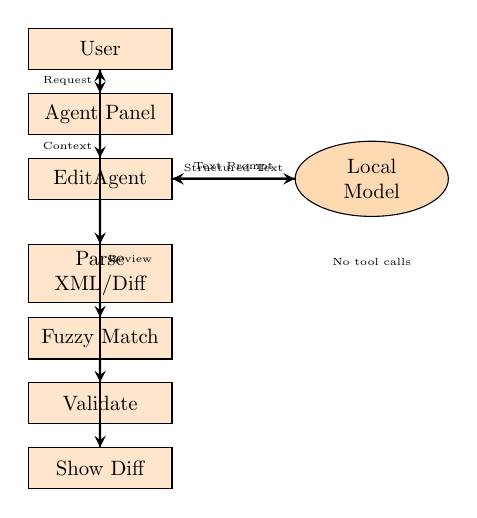
\begin{tikzpicture}[
    node distance=1.1cm,
    box/.style={rectangle, draw, text width=2.2cm, text centered, minimum height=0.7cm, fill=orange!20},
    local/.style={ellipse, draw, text width=1.6cm, text centered, minimum height=0.8cm, fill=orange!30},
    arrow/.style={->, >=stealth, thick},
    scale=0.75,
    transform shape
]
    \node[box] (user) {User};
    \node[box, below of=user] (panel) {Agent Panel};
    \node[box, below of=panel] (agent) {EditAgent};
    \node[local, right of=agent, xshift=3.5cm] (model) {Local Model};
    \node[box, below of=agent, yshift=-0.5cm] (parse) {Parse XML/Diff};
    \node[box, below of=parse] (match) {Fuzzy Match};
    \node[box, below of=match] (validate) {Validate};
    \node[box, below of=validate] (diff) {Show Diff};

    \draw[arrow] (user) -- node[left, font=\tiny] {Request} (panel);
    \draw[arrow] (panel) -- node[left, font=\tiny] {Context} (agent);
    \draw[arrow] (agent) -- node[above, font=\tiny] {Text Prompt} (model);
    \draw[arrow] (model) -- node[above, font=\tiny] {Structured Text} (agent);
    \draw[arrow] (agent) -- (parse);
    \draw[arrow] (parse) -- (match);
    \draw[arrow] (match) -- (validate);
    \draw[arrow] (validate) -- (diff);
    \draw[arrow] (diff) -- node[right, font=\tiny] {Review} (user);
    
    \node[below of=model, yshift=-0.3cm, text width=2.2cm, text centered, font=\tiny] {No tool calls};
\end{tikzpicture}
\caption{Offline Model Flow without Tool Calling}
\label{fig:offline-text}
\end{figure}

\subsection{Limitations}

Text-only mode has limitations compared to tool-calling mode:

\begin{itemize}
    \item The model cannot open additional files mid-edit
    \item All context must be provided upfront in the conversation
    \item Formatting errors in the XML or diff blocks cause rejection
    \item No multi-step autonomy (the model can't search the codebase)
\end{itemize}

However, this mode is sufficient for simple, single-file edits and works with any model that can follow the structured format.

\subsection{Configuration}

A single setting controls this behavior: \texttt{capabilities.tools: false} in the model configuration tells Zed to skip tool definitions and use text-mode prompts. This makes it easy to migrate any offline model into the smart edit flow.

\section{Edit Format Selection}

Zed automatically selects the optimal edit format based on the model. Most models use XML tags (\texttt{<old\_text>} and \texttt{<new\_text>}), but Google's Gemini models prefer diff-fenced blocks. The EditFormat is determined by checking the model's provider ID and name.

The parser handles both formats seamlessly, extracting the same structured edit information regardless of format. This allows the same fuzzy matching and application logic to work for all models.

\begin{figure}[htbp]
\centering
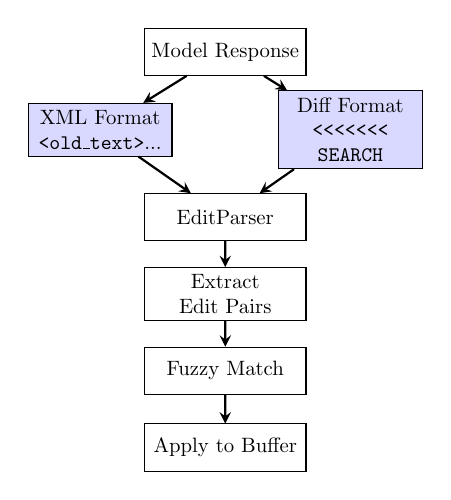
\begin{tikzpicture}[
    node distance=1.3cm,
    box/.style={rectangle, draw, text width=2.5cm, text centered, minimum height=0.8cm},
    format/.style={rectangle, draw, text width=2.2cm, text centered, minimum height=0.7cm, fill=blue!15},
    arrow/.style={->, >=stealth, thick},
    scale=0.75,
    transform shape
]
    \node[box] (model) {Model Response};
    \node[format, below left of=model, xshift=-1.2cm, yshift=-0.4cm] (xml) {XML Format\\\texttt{<old\_text>}...};
    \node[format, below right of=model, xshift=1.2cm, yshift=-0.4cm] (diff) {Diff Format\\\texttt{<<<<<<< SEARCH}};
    \node[box, below of=model, yshift=-1.5cm] (parser) {EditParser};
    \node[box, below of=parser] (extract) {Extract Edit Pairs};
    \node[box, below of=extract] (match) {Fuzzy Match};
    \node[box, below of=match] (apply) {Apply to Buffer};

    \draw[arrow] (model) -- (xml);
    \draw[arrow] (model) -- (diff);
    \draw[arrow] (xml) -- (parser);
    \draw[arrow] (diff) -- (parser);
    \draw[arrow] (parser) -- (extract);
    \draw[arrow] (extract) -- (match);
    \draw[arrow] (match) -- (apply);
\end{tikzpicture}
\caption{Edit Parsing and Application Process}
\label{fig:parsing}
\end{figure}

\section{Safety and Validation}

Zed includes several safety mechanisms:

\begin{itemize}
    \item \textbf{Path validation}: EditFileTool validates that paths are within the project before allowing edits
    \item \textbf{Authorization}: Edits to settings files or paths outside the project require user confirmation
    \item \textbf{Fuzzy matching}: The StreamingFuzzyMatcher ensures edits match actual file content, preventing hallucinations
    \item \textbf{Syntax validation}: Tree-sitter validates syntax before applying changes
    \item \textbf{Diff review}: All edits are shown in a diff view that users must explicitly accept
\end{itemize}

\section{Comparison of Model Types}

Figure~\ref{fig:comparison} illustrates the key differences between the three model deployment scenarios. While the underlying architecture remains the same, the interaction patterns and capabilities vary based on model support.

\begin{figure}[htbp]
\centering
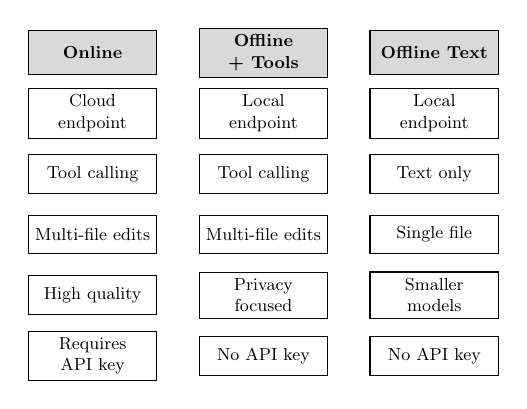
\begin{tikzpicture}[
    node distance=1.1cm,
    box/.style={rectangle, draw, text width=2.1cm, text centered, minimum height=0.7cm, font=\small},
    header/.style={rectangle, draw, text width=2.1cm, text centered, minimum height=0.8cm, fill=gray!30, font=\bfseries\small},
    scale=0.7,
    transform shape
]
    % Headers
    \node[header] (h1) {Online};
    \node[header, right of=h1, xshift=2cm] (h2) {Offline + Tools};
    \node[header, right of=h2, xshift=2cm] (h3) {Offline Text};
    
    % Online column
    \node[box, below of=h1] (o1) {Cloud endpoint};
    \node[box, below of=o1] (o2) {Tool calling};
    \node[box, below of=o2] (o3) {Multi-file edits};
    \node[box, below of=o3] (o4) {High quality};
    \node[box, below of=o4] (o5) {Requires API key};
    
    % Offline + Tools column
    \node[box, below of=h2] (t1) {Local endpoint};
    \node[box, below of=t1] (t2) {Tool calling};
    \node[box, below of=t2] (t3) {Multi-file edits};
    \node[box, below of=t3] (t4) {Privacy focused};
    \node[box, below of=t4] (t5) {No API key};
    
    % Offline Text column
    \node[box, below of=h3] (x1) {Local endpoint};
    \node[box, below of=x1] (x2) {Text only};
    \node[box, below of=x2] (x3) {Single file};
    \node[box, below of=x3] (x4) {Smaller models};
    \node[box, below of=x4] (x5) {No API key};
\end{tikzpicture}
\caption{Comparison of Three Model Deployment Scenarios}
\label{fig:comparison}
\end{figure}

\section{Conclusion}

Zed's smart edit system demonstrates a unified approach to AI-powered code editing that works across three distinct model deployment scenarios. By abstracting the differences between online and offline models, and between tool-calling and text-only models, Zed provides a consistent user experience while maximizing compatibility.

The key insight is that smart edit doesn't require tool calling—it can work with any model that can produce structured text output. This makes the feature accessible to a wide range of models, from high-end cloud services to small local models, while maintaining safety through validation and review mechanisms.

The architecture's strength lies in its flexibility: the same EditAgent, parser, and fuzzy matcher handle all three scenarios, with only the prompt format and tool availability changing based on model capabilities. This design allows Zed to provide smart edit functionality regardless of where or how the language model runs.

\end{document}

